\documentclass[./../main_file.tex]{subfiles}
\begin{document}
\subsection{Các nút và đầu nối}
\begin{figure}[H]
	\centering
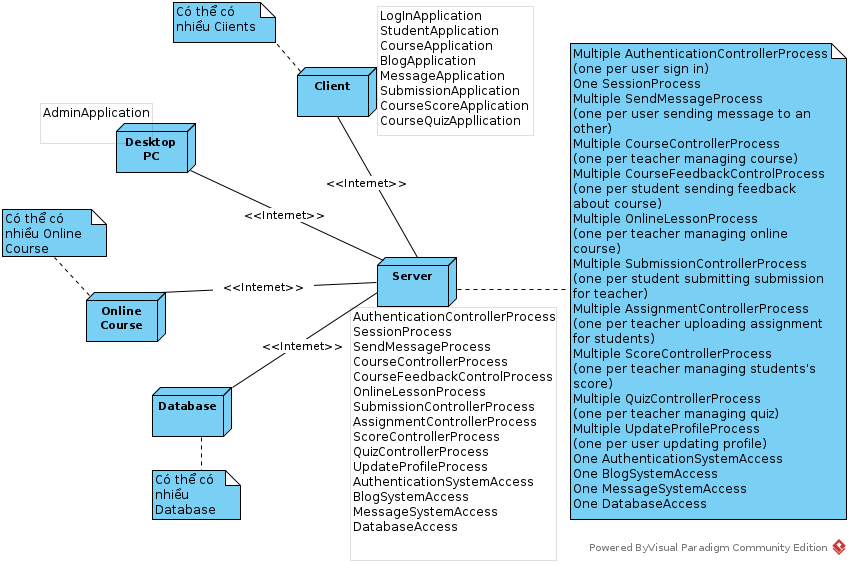
\includegraphics[width=\textwidth]{deployment_model.png}
	\caption{Biểu đồ khung nhìn triển khai}
\end{figure}
\subsection{Ánh xạ tiến trình và nút}

Các tiến trình được chạy trên Client là:
\begin{itemize}[leftmargin=+0.5in]
	\item SignInApplication
	\item SignUpApplication
	\item CourseApplication
	\item ChatApplication
\end{itemize}


Các tiến trình được chạy trên Desktop PC là:
\begin{itemize}[leftmargin=+0.5in]
	\item AdminApplication
\end{itemize}


Các tiến trình được chạy trên Server là:
\begin{itemize}[leftmargin=+0.5in]
\item AuthenticationControllerProcess
	\item UserControllerProcess
	\item SessionProcess
	\item ChatProcess
	\item LiveStreamProcess
	\item CourseControllerProcess
	\item UserFilterProcess
	\item DatabaseAccess
\end{itemize}
\end{document}